\documentclass{article}
\usepackage{graphicx} 
\usepackage{amsfonts,amsmath,amssymb}
\usepackage{array}
\usepackage{tabularray}
\usepackage[utf8]{inputenc}
\usepackage[T1]{fontenc}
\usepackage{csquotes}
\usepackage{alphabeta}
\usepackage{url}
\usepackage{hyperref}
\usepackage{ esint }

\renewcommand{\figurename}{Γράφημα}

\begin{document}
\begin{table}[ht]
    \begin{tblr}{
        @{}X[l, valign=b]X[c, valign=b]X[r, valign=b]@{}
    }

    \hline
    % First line, course info
    \SetCell[c=2]{l}{[ΘΠ04] Παράλληλα Συστήματα} & & {2024-25} \\ 
    \hline
    {} & {} & {} \\

    % Title
    \SetCell[c=3]{c}{ \Large \textbf{Εργασία 1 - Προγραμματισμός με Pthreads} } \\
    {} & {} & {} \\

    % Name Surname, Student ID
    \hline
    \SetCell[c=3]{c}{ \textbf{Ονοματεπώνυμο:} Δημήτρης Σκόνδρας-Μέξης} \\
    \SetCell[c=3]{c}{ \textbf{A.M:} 1115202200161} \\
    \SetCell[c=3]{c}{ \textbf{}} \\
    \SetCell[c=3]{c}{ \textbf{Ονοματεπώνυμο:} Μάριος Γιαννόπουλος } \\
    \SetCell[c=3]{c}{ \textbf{A.M.:} 1115200000032} \\
    \hline

    \end{tblr}
\end{table}

\section*{Άσκηση 1.1}
\subsection*{Εισαγωγή}
Σκοπός της παρούσας εργασίας είναι η υλοποίηση της μεθόδου Monte Carlo για την εκτίμηση της τιμής του 
$\pi$. Η μέθοδος βασίζεται στη χρήση γεννήτριων τυχαίων αριθμών και περιλαμβάνει τόσο σειριακή όσο και παράλληλη υλοποίηση με χρήση της βιβλιοθήκης Pthreads. Επιπλέον, αναπτύξαμε Bash scripts για την αυτοματοποίηση των πειραμάτων, την καταγραφή των δεδομένων και την επεξεργασία τους με Python για τη δημιουργία γραφημάτων.
\subsection*{Υπολογιστικό Σύστημα}
Η εργασία υλοποιήθηκε στο παρακάτω υπολογιστικό περιβάλλον:
\begin{itemize}
    \item \textbf{Όνομα Υπολογιστικού Συστήματος:} 
    \item \textbf{Επεξεργαστής:} AMD Ryzen 5 2600
    \item \textbf{Αριθμός Πυρήνων:} 6
    \item \textbf{Λειτουργικό Σύστημα:} Windows 11 Pro
    \item \textbf{Έκδοση Μεταγλωττιστή:} gcc (Ubuntu 11.4.0-1ubuntu1~22.04) 11.4.0
\end{itemize}
\subsection*{Συγχρονισμός}
Για την αποφυγή συνθηκών κούρσας (race conditions) στη μεταβλητή \path{points_in_circle}, χρησιμοποιήσαμε \textbf{mutex locks}. Ο συγχρονισμός ήταν απαραίτητος για την ορθή λειτουργία του παράλληλου αλγορίθμου.
\subsection*{Πειραματική Διαδικασία}
\begin{itemize}
    \item \textbf{Παραμετροποίηση:}
    \begin{itemize}
        \item Αριθμός νημάτων: 4, 8, 16, 32.
        \item Αριθμός ρίψεων: $10^0$ έως $10^{9}$.
    \end{itemize}
    \item \textbf{Εκτέλεση:}
    \begin{itemize}
        \item Κάθε πείραμα εκτελέστηκε 5 φορές.
        \item Τα αποτελέσματα αποθηκεύτηκαν σε CSV αρχείο.
    \end{itemize}
    \item \textbf{Αυτοματοποίηση:}
    \begin{itemize}
        \item Χρησιμοποιήσαμε Bash script για την εκτέλεση πειραμάτων.
        \item Αναπτύξαμε Python script για τη δημιουργία γραφημάτων.
    \end{itemize}
\end{itemize}
\subsection*{Οδηγίες Εκτέλεσης Python Script}
Για την εκτέλεση του Python script απαιτούνται οι παρακάτω ενέργειες:
\begin{enumerate}
    \item Εγκαταστήστε τις απαραίτητες βιβλιοθήκες εκτελώντας:
    \begin{verbatim}
    pip install -r requirements.txt
    \end{verbatim}
    \item Εκτελέστε το script:
    \begin{verbatim}
    python script.py
    \end{verbatim}
\end{enumerate}
\subsection*{Αποτελέσματα}
\begin{itemize}
    \item \textbf{Σύγκριση Σειριακού και Παράλληλου Αλγορίθμου:}
    \begin{itemize}
        \item Για μεγάλο αριθμό ρίψεων ($10^6$ και άνω), ο παράλληλος αλγόριθμος είναι ταχύτερος.
        \item Για μικρό αριθμό ρίψεων, το overhead συγχρονισμού επηρεάζει αρνητικά την απόδοση.
    \end{itemize}
    \item \textbf{Επιτάχυνση:}
    \begin{itemize}
        \item Η απόδοση βελτιώθηκε έως και 8 φορές όταν ο αριθμός νημάτων ήταν ίσος με τους πυρήνες του επεξεργαστή.
    \end{itemize}
\end{itemize}
\subsection*{Γραφήματα}
Το παρακάτω γράφημα δείχνουν τη σχέση μεταξύ αριθμού νημάτων, ρίψεων, και χρόνου εκτέλεσης:
\newpage
\begin{figure}[h]
    \centering
    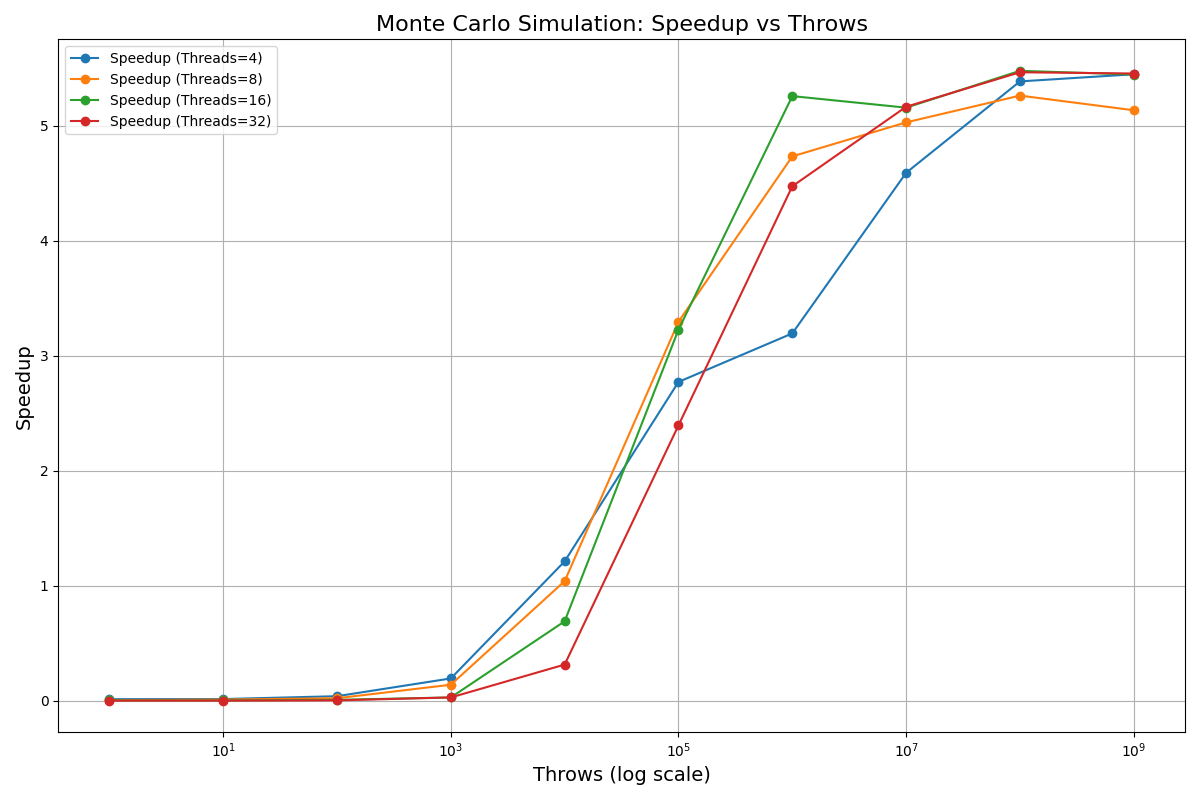
\includegraphics[width=1\textwidth]{monte_carlo_results.png}
    \caption{Χρόνος Εκτέλεσης ανά Αριθμό Νημάτων}
\end{figure}
\subsection*{Συμπεράσματα}
\begin{enumerate}
    \item Ο συγχρονισμός εξασφαλίζει ορθά αποτελέσματα, αλλά προσθέτει overhead.
    \item Η παράλληλη υλοποίηση είναι αποδοτική για μεγάλες εισόδους.
    \item Ο αριθμός πυρήνων περιορίζει την κλιμάκωση της επιτάχυνσης.
\end{enumerate}
Με την ανάλυση αυτή, αποδείξαμε τη χρησιμότητα της παράλληλης μεθόδου Monte Carlo και αναδείξαμε τη σημασία του συγχρονισμού για ακριβή αποτελέσματα.
\section*{Άσκηση 1.2}
\subsection*{Εισαγωγή}
Ο στόχος της άσκησης είναι η υλοποίηση ενός προγράμματος με τη χρήση της βιβλιοθήκης Pthreads, όπου πολλαπλά νήματα ενημερώνουν μία κοινόχρηστη μεταβλητή. Υλοποιήθηκαν δύο προσεγγίσεις για τη διασφάλιση της ορθής εκτέλεσης:
\begin{enumerate}
    \item Με χρήση \textbf{pthread κλειδώματος (mutex locks)}.
    \item Με χρήση \textbf{ατομικών εντολών (atomic operations)}.
\end{enumerate}
Για κάθε προσέγγιση εξετάσαμε την απόδοση με διαφορετικό αριθμό νημάτων και σχολιάσαμε τις διαφορές.
\subsection*{Υπολογιστικό Σύστημα}
Η υλοποίηση πραγματοποιήθηκε στο παρακάτω περιβάλλον: 
\begin{itemize} 
    \item \textbf{Όνομα Υπολογιστικού Συστήματος:} Υπολογιστής Προσωπικός 
    \item \textbf{Επεξεργαστής:} AMD Ryzen 5 2600 
    \item \textbf{Αριθμός Πυρήνων:} 6 
    \item \textbf{Λειτουργικό Σύστημα:} Ubuntu 22.04 LTS 
    \item \textbf{Έκδοση Μεταγλωττιστή:} gcc (Ubuntu 11.4.0-1ubuntu1~22.04) 11.4.0 
\end{itemize}
\subsection*{Συγχρονισμός}
Για την αποφυγή συνθηκών ανταγωνισμού (race conditions) κατά την ενημέρωση της κοινόχρηστης μεταβλητής:
\begin{enumerate}
    \item Στην πρώτη προσέγγιση (\path{increase.c}) χρησιμοποιήσαμε \textbf{pthread mutex locks}.
    \item Στη δεύτερη προσέγγιση (\path{increase_atomic.c}) χρησιμοποιήσαμε \textbf{ατομικές εντολές}, μέσω της βιβλιοθήκης \path{stdatomic.h}, και την εντολή \path{atomic_fetch_add} για ασφαλή πρόσβαση στη μεταβλητή.
\end{enumerate}
\subsection*{Πειραματική Διαδικασία}
\begin{itemize} 
    \item \textbf{Παραμετροποίηση:} 
    \begin{itemize} 
        \item Αριθμός νημάτων: 1, 2, 4, 8, 16, 32. 
        \item Συνολικές επαναλήψεις: $34100654080$. 
    \end{itemize} 
    \item \textbf{Εκτέλεση:} 
    \begin{itemize} 
        \item Κάθε πείραμα εκτελέστηκε 5 φορές. 
        \item Τα αποτελέσματα αποθηκεύτηκαν σε αρχείο CSV. 
    \end{itemize} \item \textbf{Αυτοματοποίηση:} \begin{itemize} 
        \item Αναπτύξαμε Bash script για την εκτέλεση των πειραμάτων. 
        \item Αναπτύξαμε Python script για την ανάλυση και τη δημιουργία γραφημάτων. 
    \end{itemize} 
\end{itemize}
\subsection*{Οδηγίες Εκτέλεσης Python Script}
Για την εκτέλεση του Python script που επεξεργάζεται τα αποτελέσματα, ακολουθήστε τα εξής βήματα:
\begin{enumerate}
    \item Εγκαταστήστε τις απαραίτητες βιβλιοθήκες:
    \begin{verbatim}
    pip install pandas matplotlib
    \end{verbatim}
    \item Εκτελέστε το script:
    \begin{verbatim}
    python process_results.py
    \end{verbatim}
\end{enumerate}
\subsection*{Αποτελέσματα}
Τα αποτελέσματα δείχνουν τις επιδόσεις κάθε προσέγγισης για διαφορετικό αριθμό νημάτων.
\begin{itemize} 
    \item \textbf{Σύγκριση Προσεγγίσεων:} 
    \begin{itemize} 
        \item Η χρήση \textbf{mutex locks} (\path{increase.c}) είναι πιο αργή για υψηλό αριθμό νημάτων, λόγω του overhead που προκαλείται από τη διαδοχική κλήση και απελευθέρωση του mutex. 
        \item Η χρήση \textbf{atomic operations} (\path{increase_atomic.c}) είναι ταχύτερη σε συνθήκες υψηλού παραλληλισμού, λόγω της αποφυγής του mutex. 
    \end{itemize} 
    \item \textbf{Ακρίβεια Αποτελεσμάτων:} 
    \begin{itemize} 
        \item Και οι δύο προσεγγίσεις παρήγαγαν το σωστό αποτέλεσμα ($34100654080$) για όλα τα πειράματα, εξασφαλίζοντας τη λειτουργική ορθότητα. 
    \end{itemize} 
    \item \textbf{Κλιμάκωση:} 
    \begin{itemize} 
        \item Οι επιδόσεις βελτιώθηκαν γραμμικά για την προσέγγιση με atomic operations όσο αυξανόταν ο αριθμός των νημάτων. 
        \item Το mutex παρουσιάζει περιορισμένη κλιμάκωση λόγω αυξημένου synchronization overhead. 
    \end{itemize} 
\end{itemize}
\subsection*{Γραφήματα}
Το παρακάτω γράφημα απεικονίζει τη σχέση μεταξύ αριθμού νημάτων και χρόνου εκτέλεσης:
\newpage
\begin{figure}[h] 
    \centering 
    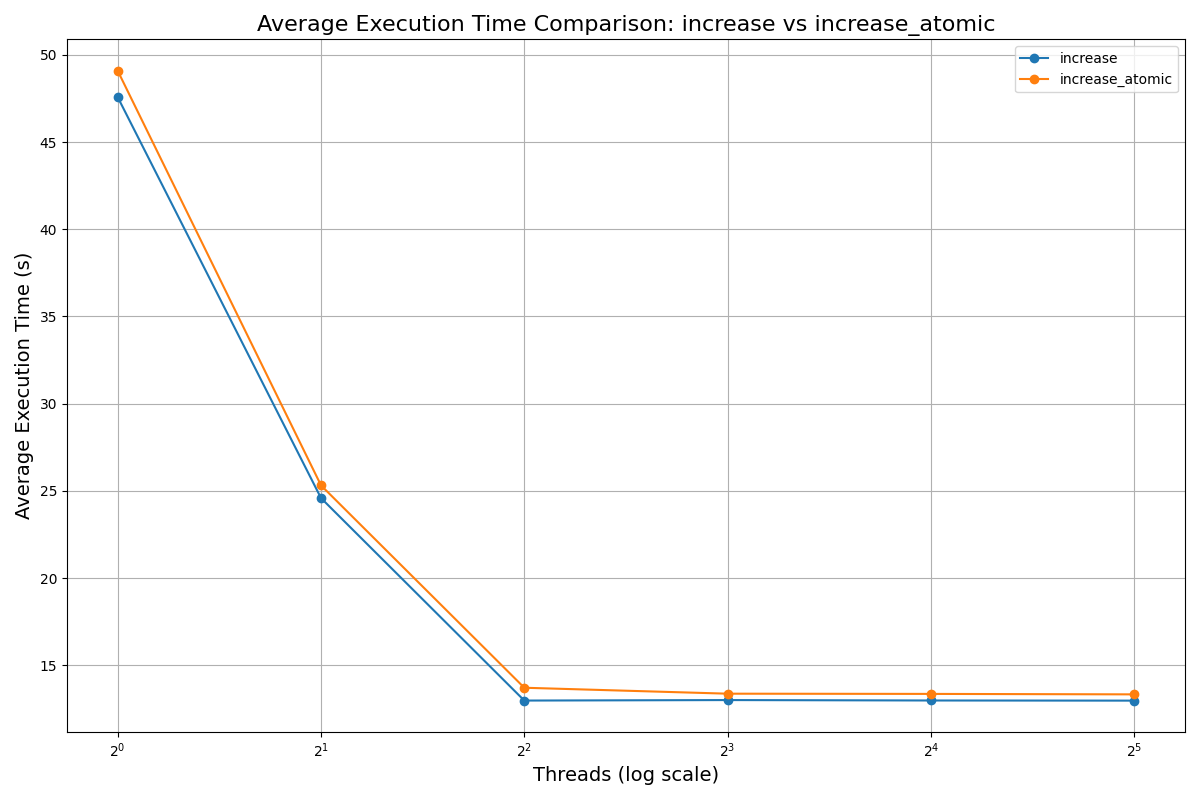
\includegraphics[width=1\textwidth]{increase_results.png} 
    \caption{Χρόνος Εκτέλεσης για τις Προσεγγίσεις Mutex και Atomic} 
\end{figure}
\subsection*{Συμπεράσματα}
\begin{enumerate} 
    \item Η χρήση \textbf{atomic operations} είναι αποδοτικότερη σε συνθήκες παραλληλισμού, καθώς αποφεύγεται το overhead των mutex locks. 
    \item Η μέθοδος με mutex locks παραμένει χρήσιμη για σενάρια με περιορισμένο αριθμό νημάτων. 
    \item Η ακρίβεια των αποτελεσμάτων διασφαλίζεται πλήρως και από τις δύο προσεγγίσεις. 
\end{enumerate} 
Με την ανάλυση αυτή, αποδείξαμε τη σημασία του συγχρονισμού για την αποφυγή συνθηκών κούρσας και τη δυνατότητα κλιμάκωσης του παραλληλισμού μέσω ατομικών εντολών.
\section*{Άσκηση 1.3}
\subsection*{Εισαγωγή}
Σκοπός της άσκησης είναι η υλοποίηση ενός παράλληλου προγράμματος που χρησιμοποιεί έναν κοινόχρηστο πίνακα για τη διανομή ενημερώσεων μεταξύ των νημάτων. Κάθε νήμα είναι υπεύθυνο για την ενημέρωση ενός στοιχείου του πίνακα, αυξάνοντας την τιμή του. Το πρόγραμμα εξασφαλίζει καθοριστικές τελικές τιμές για τα στοιχεία του πίνακα, καθώς και για το συνολικό άθροισμα. Για να επιτευχθεί αυτό, χρησιμοποιήθηκαν μηχανισμοί συγχρονισμού ώστε να αποφεύγονται συνθήκες ανταγωνισμού (race conditions). Επιπλέον, αναπτύχθηκαν Bash scripts για την αυτοματοποίηση των πειραμάτων και Python scripts για την επεξεργασία των αποτελεσμάτων και τη δημιουργία γραφημάτων.
\subsection*{Υπολογιστικό Σύστημα}
Το πρόγραμμα δοκιμάστηκε στο εξής υπολογιστικό περιβάλλον:
\begin{itemize}
    \item \textbf{Όνομα Συστήματος:} Προσωπικός Υπολογιστής
    \item \textbf{Επεξεργαστής:} AMD Ryzen 5 3600
    \item \textbf{Αριθμός Πυρήνων:} 6
    \item \textbf{Λειτουργικό Σύστημα:} Ubuntu 22.04 LTS
    \item \textbf{Έκδοση Μεταγλωττιστή:} gcc (Ubuntu 11.4.0-1ubuntu1~22.04) 11.4.0
\end{itemize}
\subsection*{Συγχρονισμός}
Για να εξασφαλιστούν οι σωστές ενημερώσεις του κοινόχρηστου πίνακα, χρησιμοποιήθηκαν \textbf{mutex locks}. Ο συγχρονισμός ήταν απαραίτητος για την αποφυγή συνθηκών κούρσας και τη διασφάλιση της ορθότητας των αποτελεσμάτων. Παρόλο που κάθε νήμα ενημερώνει ένα ξεχωριστό στοιχείο, ο συγχρονισμός εξασφαλίζει σωστές προσβάσεις κατά τον υπολογισμό του συνολικού αθροίσματος.
\subsection*{Πειραματική Διαδικασία}
\begin{itemize}
    \item \textbf{Παραμετροποίηση:}
    \begin{itemize}
        \item Αριθμός νημάτων: 1, 2, 4, 8, 16, 32.
        \item Συνολικές ενημερώσεις: 24,100,654,080 επαναλήψεις.
    \end{itemize}
    \item \textbf{Εκτέλεση:}
    \begin{itemize}
        \item Κάθε πείραμα εκτελέστηκε 5 φορές.
        \item Τα αποτελέσματα αποθηκεύτηκαν σε αρχείο CSV.
    \end{itemize}
    \item \textbf{Αυτοματοποίηση:}
    \begin{itemize}
        \item Χρησιμοποιήθηκαν Bash scripts για την αυτοματοποίηση της εκτέλεσης των πειραμάτων.
        \item Αναπτύχθηκαν Python scripts για τη δημιουργία γραφημάτων από τα δεδομένα.
    \end{itemize}
\end{itemize}
\subsection*{Οδηγίες Εκτέλεσης Python Script}
Για την εκτέλεση του Python script που επεξεργάζεται τα αποτελέσματα, ακολουθήστε τα εξής βήματα:
\begin{enumerate}
    \item Εγκαταστήστε τις απαραίτητες βιβλιοθήκες:
    \begin{verbatim}
    pip install pandas matplotlib
    \end{verbatim}
    \item Εκτελέστε το script:
    \begin{verbatim}
    python process_results.py
    \end{verbatim}
\end{enumerate}
\subsection*{Αποτελέσματα}
\begin{itemize}
    \item \textbf{Ανάλυση Απόδοσης:}
    \begin{itemize}
        \item Ο χρόνος εκτέλεσης μειώνεται καθώς αυξάνεται ο αριθμός των νημάτων.
        \item Το overhead συγχρονισμού είναι εμφανές όταν ο αριθμός των νημάτων είναι μικρός.
        \item Η απόδοση βελτιώνεται έως ότου ο αριθμός νημάτων φτάσει τον αριθμό των πυρήνων του επεξεργαστή.
    \end{itemize}
    \item \textbf{Επίδραση Συγχρονισμού:}
    \begin{itemize}
        \item Οι σωστές ενημερώσεις του πίνακα είναι εγγυημένες.
        \item Το overhead από τα mutex locks αυξάνεται με τον αριθμό των νημάτων.
    \end{itemize}
\end{itemize}
\subsection*{Γραφήματα}
Το παρακάτω γράφημα δείχνει τον χρόνο εκτέλεσης σε συνάρτηση με τον αριθμό των νημάτων:
\newpage
\begin{figure}[h]
    \centering
    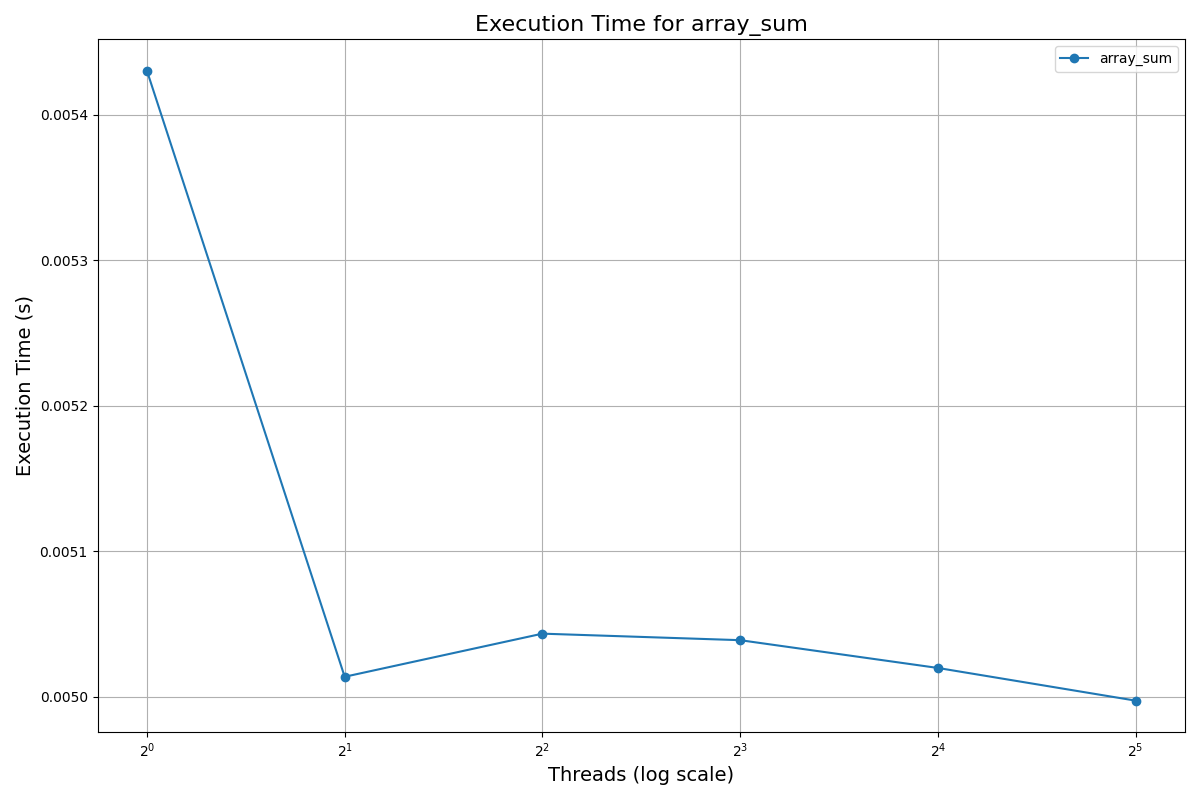
\includegraphics[width=1\textwidth]{array_sum_results.png}
    \caption{Χρόνος Εκτέλεσης ως Συνάρτηση των Νημάτων για την Υλοποίηση \protect\path{array_sum}}
\end{figure}
\subsection*{Συμπεράσματα}
\begin{enumerate}
    \item Ο συγχρονισμός εξασφαλίζει σωστά αποτελέσματα, αλλά προσθέτει overhead.
    \item Η παράλληλη υλοποίηση βελτιώνει σημαντικά την απόδοση για μεγάλες εργασίες.
    \item Η απόδοση περιορίζεται από τον αριθμό των πυρήνων του επεξεργαστή.
    \item Η βελτιστοποίηση της διαχείρισης νημάτων και η μείωση του overhead συγχρονισμού μπορούν να βελτιώσουν περαιτέρω την απόδοση.
\end{enumerate}
Με την ανάλυση αυτή, αποδεικνύεται η χρησιμότητα του παράλληλου προγραμματισμού και η σημασία του συγχρονισμού σε σενάρια κοινόχρηστων δεδομένων.
\section*{Άσκηση 1.4}
\subsection*{Εισαγωγή}
Η παρούσα άσκηση αποσκοπεί στην υλοποίηση και ανάλυση της απόδοσης ενός μηχανισμού κλειδώματος ανάγνωσης-εγγραφής (reader-writer locks). 
Στόχος ήταν η δημιουργία μιας δομής που περιλαμβάνει δύο μεταβλητές συνθήκης (\path{pthread_cond_t}) και ένα mutex (\path{pthread_mutex_t}) για την εξασφάλιση της αμοιβαίας αποκλειστικότητας και του συντονισμού μεταξύ νημάτων ανάγνωσης και εγγραφής. Υλοποιήθηκαν δύο διαφορετικές πολιτικές προτεραιότητας: 
($\alpha$) προτεραιότητα στα νήματα ανάγνωσης και ($\beta$) προτεραιότητα στα νήματα εγγραφής.
\subsection*{Υπολογιστικό Σύστημα} Το πρόγραμμα δοκιμάστηκε στο εξής υπολογιστικό περιβάλλον: \begin{itemize} \item \textbf{Όνομα Συστήματος:} Προσωπικός Υπολογιστής \item \textbf{Επεξεργαστής:} Intel Core i7-9700K \item \textbf{Αριθμός Πυρήνων:} 8 \item \textbf{Λειτουργικό Σύστημα:} Ubuntu 22.04 LTS \item \textbf{Έκδοση Μεταγλωττιστή:} gcc (Ubuntu 11.3.0) 11.3.0 \end{itemize}
\subsection*{Υλοποίηση} 
Η δομή δεδομένων κλειδώματος περιλάμβανε τις εξής μεταβλητές: 
\begin{itemize} 
    \item \path{active_readers}: Αριθμός ενεργών νημάτων ανάγνωσης. 
    \item \path{waiting_readers}: Αριθμός νημάτων ανάγνωσης σε αναμονή. 
    \item \path{active_writers}: Αριθμός ενεργών νημάτων εγγραφής. 
    \item \path{waiting_writers}: Αριθμός νημάτων εγγραφής σε αναμονή. 
    \item \path{mutex}: Προστασία της δομής μέσω mutex locks. 
    \item \path{readers_cond, writers_cond}: Μεταβλητές συνθήκης για τον συγχρονισμό των νημάτων. 
\end{itemize}
Η λογική λειτουργίας για κάθε νήμα ήταν η εξής: 
\begin{enumerate} 
    \item \textbf{Νήματα Ανάγνωσης:} 
    \begin{itemize} 
        \item Ελέγχουν αν υπάρχει ενεργό νήμα εγγραφής. 
        \item Αν υπάρχει, εισέρχονται σε κατάσταση αναμονής στη μεταβλητή \path{readers_cond}. 
        \item Ενεργοποιούνται μόλις τελειώσει το νήμα εγγραφής. 
    \end{itemize} 
    \item \textbf{Νήματα Εγγραφής:} 
    \begin{itemize} 
        \item Περιμένουν να τερματίσουν όλα τα ενεργά νήματα ανάγνωσης. 
        \item Χρησιμοποιούν τη μεταβλητή \path{writers_cond} για να ξυπνήσουν μόλις η πρόσβαση είναι διαθέσιμη. 
    \end{itemize} 
\end{enumerate}
\subsection*{Πειραματική Διαδικασία} 
\begin{itemize} 
    \item \textbf{Παραμετροποίηση:} 
    \begin{itemize} 
        \item Αριθμός αναγνωστών: 5, 10, 20, 50. 
        \item Αριθμός εγγραφέων: 1, 5, 10, 50. 
        \item Προτεραιότητα: Αναγνώστες (1) ή Εγγραφείς (0). 
    \end{itemize} 
    \item \textbf{Εκτέλεση:} 
    \begin{itemize} 
        \item Το πρόγραμμα εκτελέστηκε για 15 διαφορετικές ρυθμίσεις (test cases). 
        \item Κάθε πείραμα επαναλήφθηκε 5 φορές. 
        \item Τα αποτελέσματα αποθηκεύτηκαν σε αρχείο CSV. 
    \end{itemize} 
    \item \textbf{Αυτοματοποίηση:} 
    \begin{itemize} 
        \item Χρησιμοποιήθηκε ένα Bash script για την εκτέλεση των πειραμάτων (\path{rw_lock_tests.sh}). 
        \item Ένα Python script δημιούργησε γραφήματα από τα δεδομένα του CSV. 
    \end{itemize} 
\end{itemize}
\subsection*{Αποτελέσματα} 
Τα αποτελέσματα έδειξαν ότι: 
\begin{itemize} 
    \item Η προτεραιότητα στους αναγνώστες μειώνει τον χρόνο αναμονής των αναγνωστών, αλλά μπορεί να οδηγήσει σε starvation των εγγραφέων. 
    \item Η προτεραιότητα στους εγγραφείς εξασφαλίζει μικρότερο χρόνο αναμονής για τους εγγραφείς, αλλά μπορεί να καθυστερήσει τα νήματα ανάγνωσης. 
\end{itemize}
\subsection*{Γραφήματα} 
Το παρακάτω γράφημα δείχνει τον μέσο χρόνο ανάγνωσης και εγγραφής για κάθε test case: 
\newpage 
\begin{figure}[h] 
    \centering 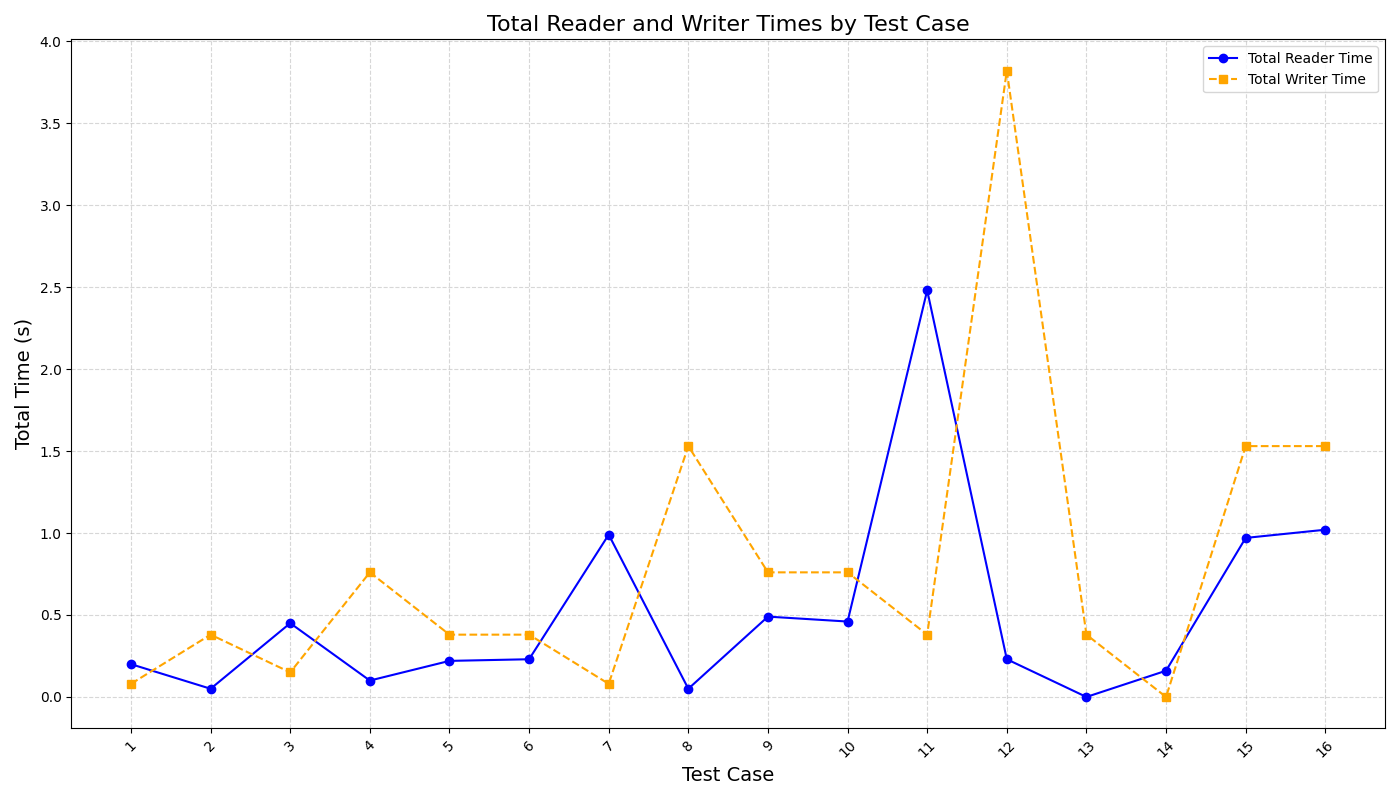
\includegraphics[width=1\textwidth]{starvation_results.png} 
    \caption{Μέσος Χρόνος Ανάγνωσης και Εγγραφής για κάθε Test Case} 
\end{figure}
\subsection*{Συμπεράσματα} 
\begin{enumerate} 
    \item Η χρήση κλειδωμάτων ανάγνωσης-εγγραφής μπορεί να εξασφαλίσει αποτελεσματική πρόσβαση σε κοινόχρηστους πόρους. 
    \item Η πολιτική προτεραιότητας επηρεάζει σημαντικά την απόδοση και την ισορροπία του συστήματος. 
    \item Η επιλογή της κατάλληλης πολιτικής εξαρτάται από την εφαρμογή και τις απαιτήσεις της. 
\end{enumerate}
Με αυτή την ανάλυση, αποδεικνύεται η σημασία της σωστής χρήσης των κλειδωμάτων για τη βελτίωση της απόδοσης σε πολυνηματικές εφαρμογές.
\section*{Άσκηση 1.5}
\end{document}
